\documentclass[12pt, letterpaper]{article}
\usepackage[utf8]{inputenc}
\usepackage{graphicx}
\usepackage{caption}
\usepackage{subcaption}
\usepackage{geometry}
\usepackage{float}
\usepackage{amsmath}
\usepackage{fancyhdr}
\usepackage{pdfpages} % Required for inserting the CamScanner PDF

% Page Geometry
\geometry{margin=1in}
\setlength{\headheight}{14.49998pt}
\addtolength{\topmargin}{-2.49998pt}

\graphicspath{{./Pictures/}}
\pdfcompresslevel=9
\pdfobjcompresslevel=3
\pdfminorversion=5

% Header/Footer Setup
\pagestyle{fancy}
\fancyhf{}
\lhead{EEE3307: Lab 3 Report}
\rhead{Yousef Awad}
\cfoot{\thepage}

\title{
    \vspace{1in}
    \textbf{\huge EEE3307 Electronics I} \\[0.5em]
    \textbf{\Large Experiment \#3: Transistor Biasing}
    \vspace{1.5in}
}
\author{
    \textbf{Name:} Yousef Alaa Awad \\
    \textbf{Partners:} Egor Shevchenko and Abram Tadros
}
\date{Lab Session: February 19, 2026}

\begin{document}

\maketitle
\newpage

%----------------------------------------------------------------------------------------
%	1. INTRODUCTION
%----------------------------------------------------------------------------------------
\section{Introduction}
The primary objective of this experiment was to study transistor biasing and bias stability within amplifier circuits. Proper biasing is necessary to establish a stable DC operating point, or Q-point, on the transistor's load line. When an AC input signal is applied, it disturbs the base current, which in turn causes the Q-point to move along the load line and produces a proportionally larger disturbance in the collector current, achieving signal amplification. 

%----------------------------------------------------------------------------------------
%	2. PROCEDURE
%----------------------------------------------------------------------------------------
\section{Experimental Procedure}
This experiment utilized 2N2222 Bipolar Transistors, resistors, capacitors, and standard laboratory equipment. Measurements and signal generation were performed using a Tektronix DPO 4034 Digital Oscilloscope, a Tektronix AFG3022 Dual Channel Function Generator, and a DC Power Supply.

The experiment was divided into several stages:
\begin{enumerate}
    \item \textbf{Fixed Bias Circuit:} The circuit corresponding to Figure 1.b in the lab manual was constructed using $R_C = 1.8 \text{ k}\Omega$, $R_B = 5.6 \text{ k}\Omega$, and $R_E = 0 \ \Omega$. The Q-point values $I_{CQ}$ and $V_{CEQ}$ were measured. 
    \item \textbf{Addition of Emitter Resistor:} The circuit was modified by inserting an emitter resistor $R_E = 1.8 \text{ k}\Omega$ to observe changes in bias stability. 
    \item \textbf{Voltage-Divider Bias with AC Input:} The circuit in Figure 3 of the lab manual was constructed with $R_C = R_E = 1.8 \text{ k}\Omega$. A $3 \text{ kHz}$ sinusoidal signal was applied to the input through a $10 \ \mu\text{F}$ coupling capacitor. The amplitude was adjusted to prevent waveform clipping, and the input ($v_i$), collector ($v_c$), and emitter ($v_e$) voltages were recorded.
\end{enumerate}

\pagebreak
%----------------------------------------------------------------------------------------
%	3. RESULTS AND DISCUSSION
%----------------------------------------------------------------------------------------
\section{Results and Discussion}

\subsection{Transistor Biasing Without Emitter Resistor (Fig. 1.b)}
For the standard fixed-bias configuration ($R_E = 0 \ \Omega$), the DC operating point was measured using a digital multimeter. The measured collector current ($I_{CQ}$) was $3.3816 \text{ mA}$ (Figure \ref{fig:icq_no_re}), and the measured collector-emitter voltage ($V_{CEQ}$) was $5.9474 \text{ V}$ (Figure \ref{fig:vceq_no_re}). 

\begin{figure}[H]
    \centering
    \begin{subfigure}[b]{0.48\textwidth}
        \centering
        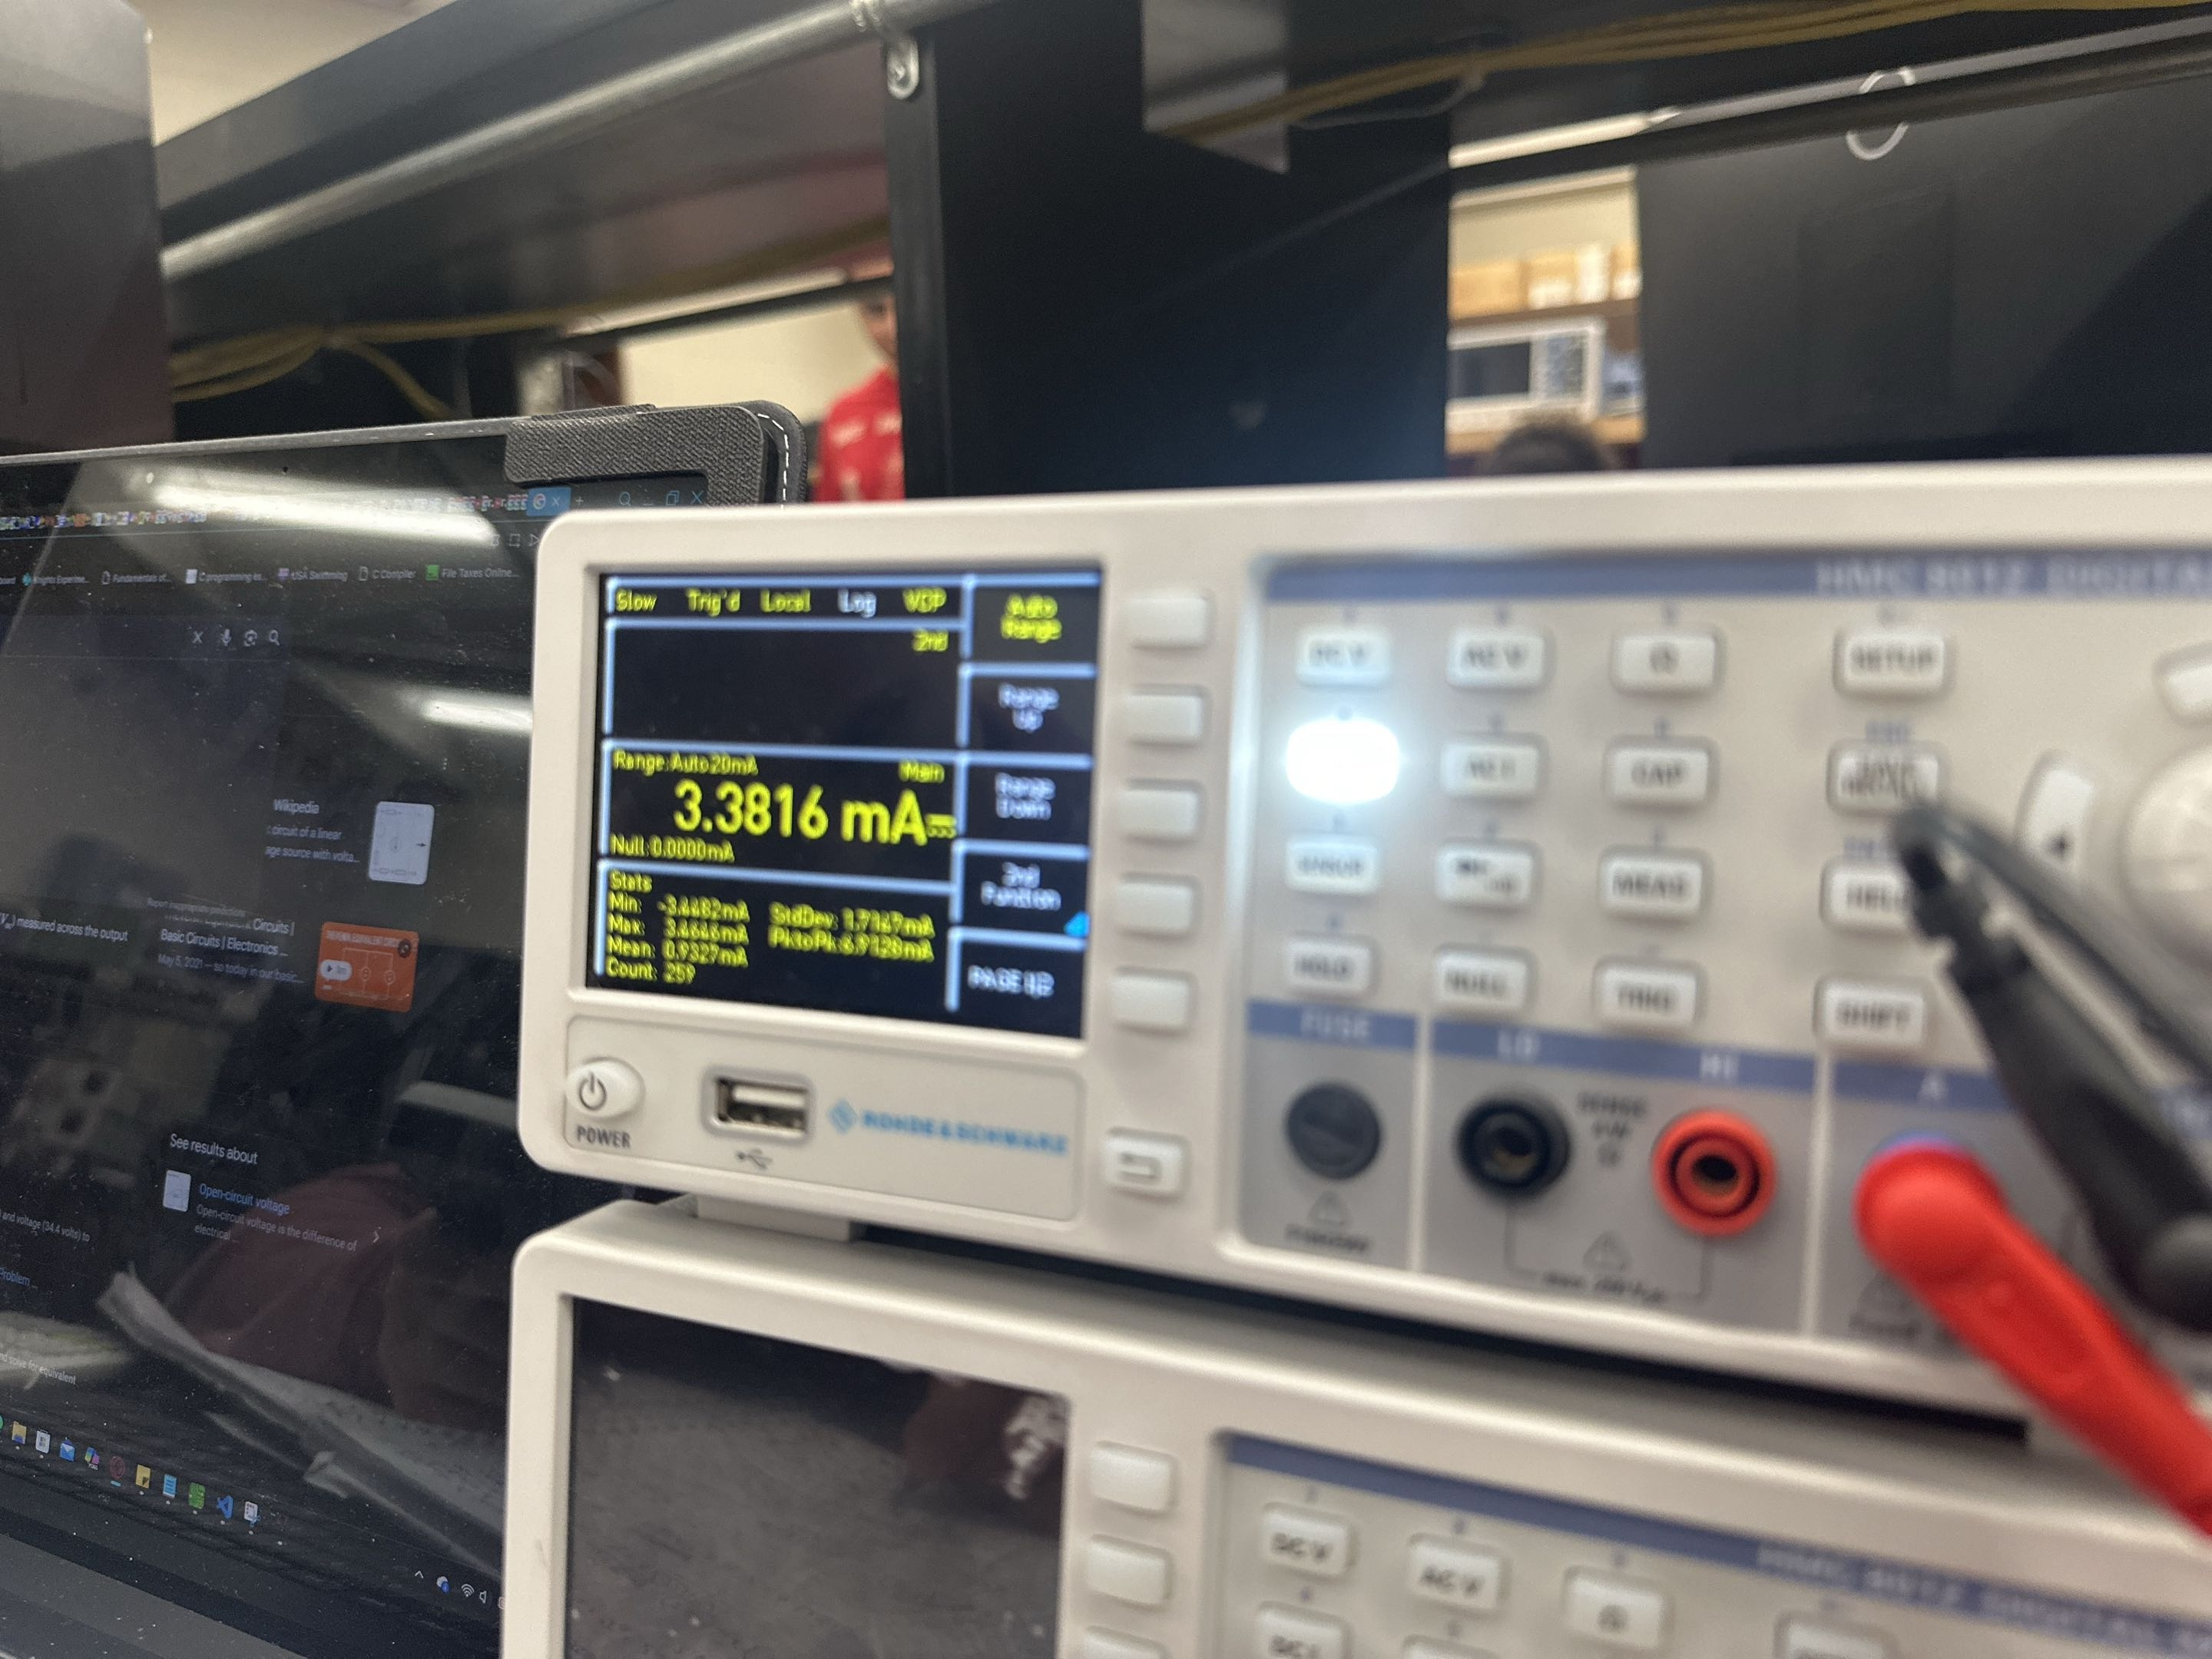
\includegraphics[width=\textwidth]{icq_figure1b.jpg}
        \caption{Measured $I_{CQ}$}
        \label{fig:icq_no_re}
    \end{subfigure}
    \hfill
    \begin{subfigure}[b]{0.48\textwidth}
        \centering
        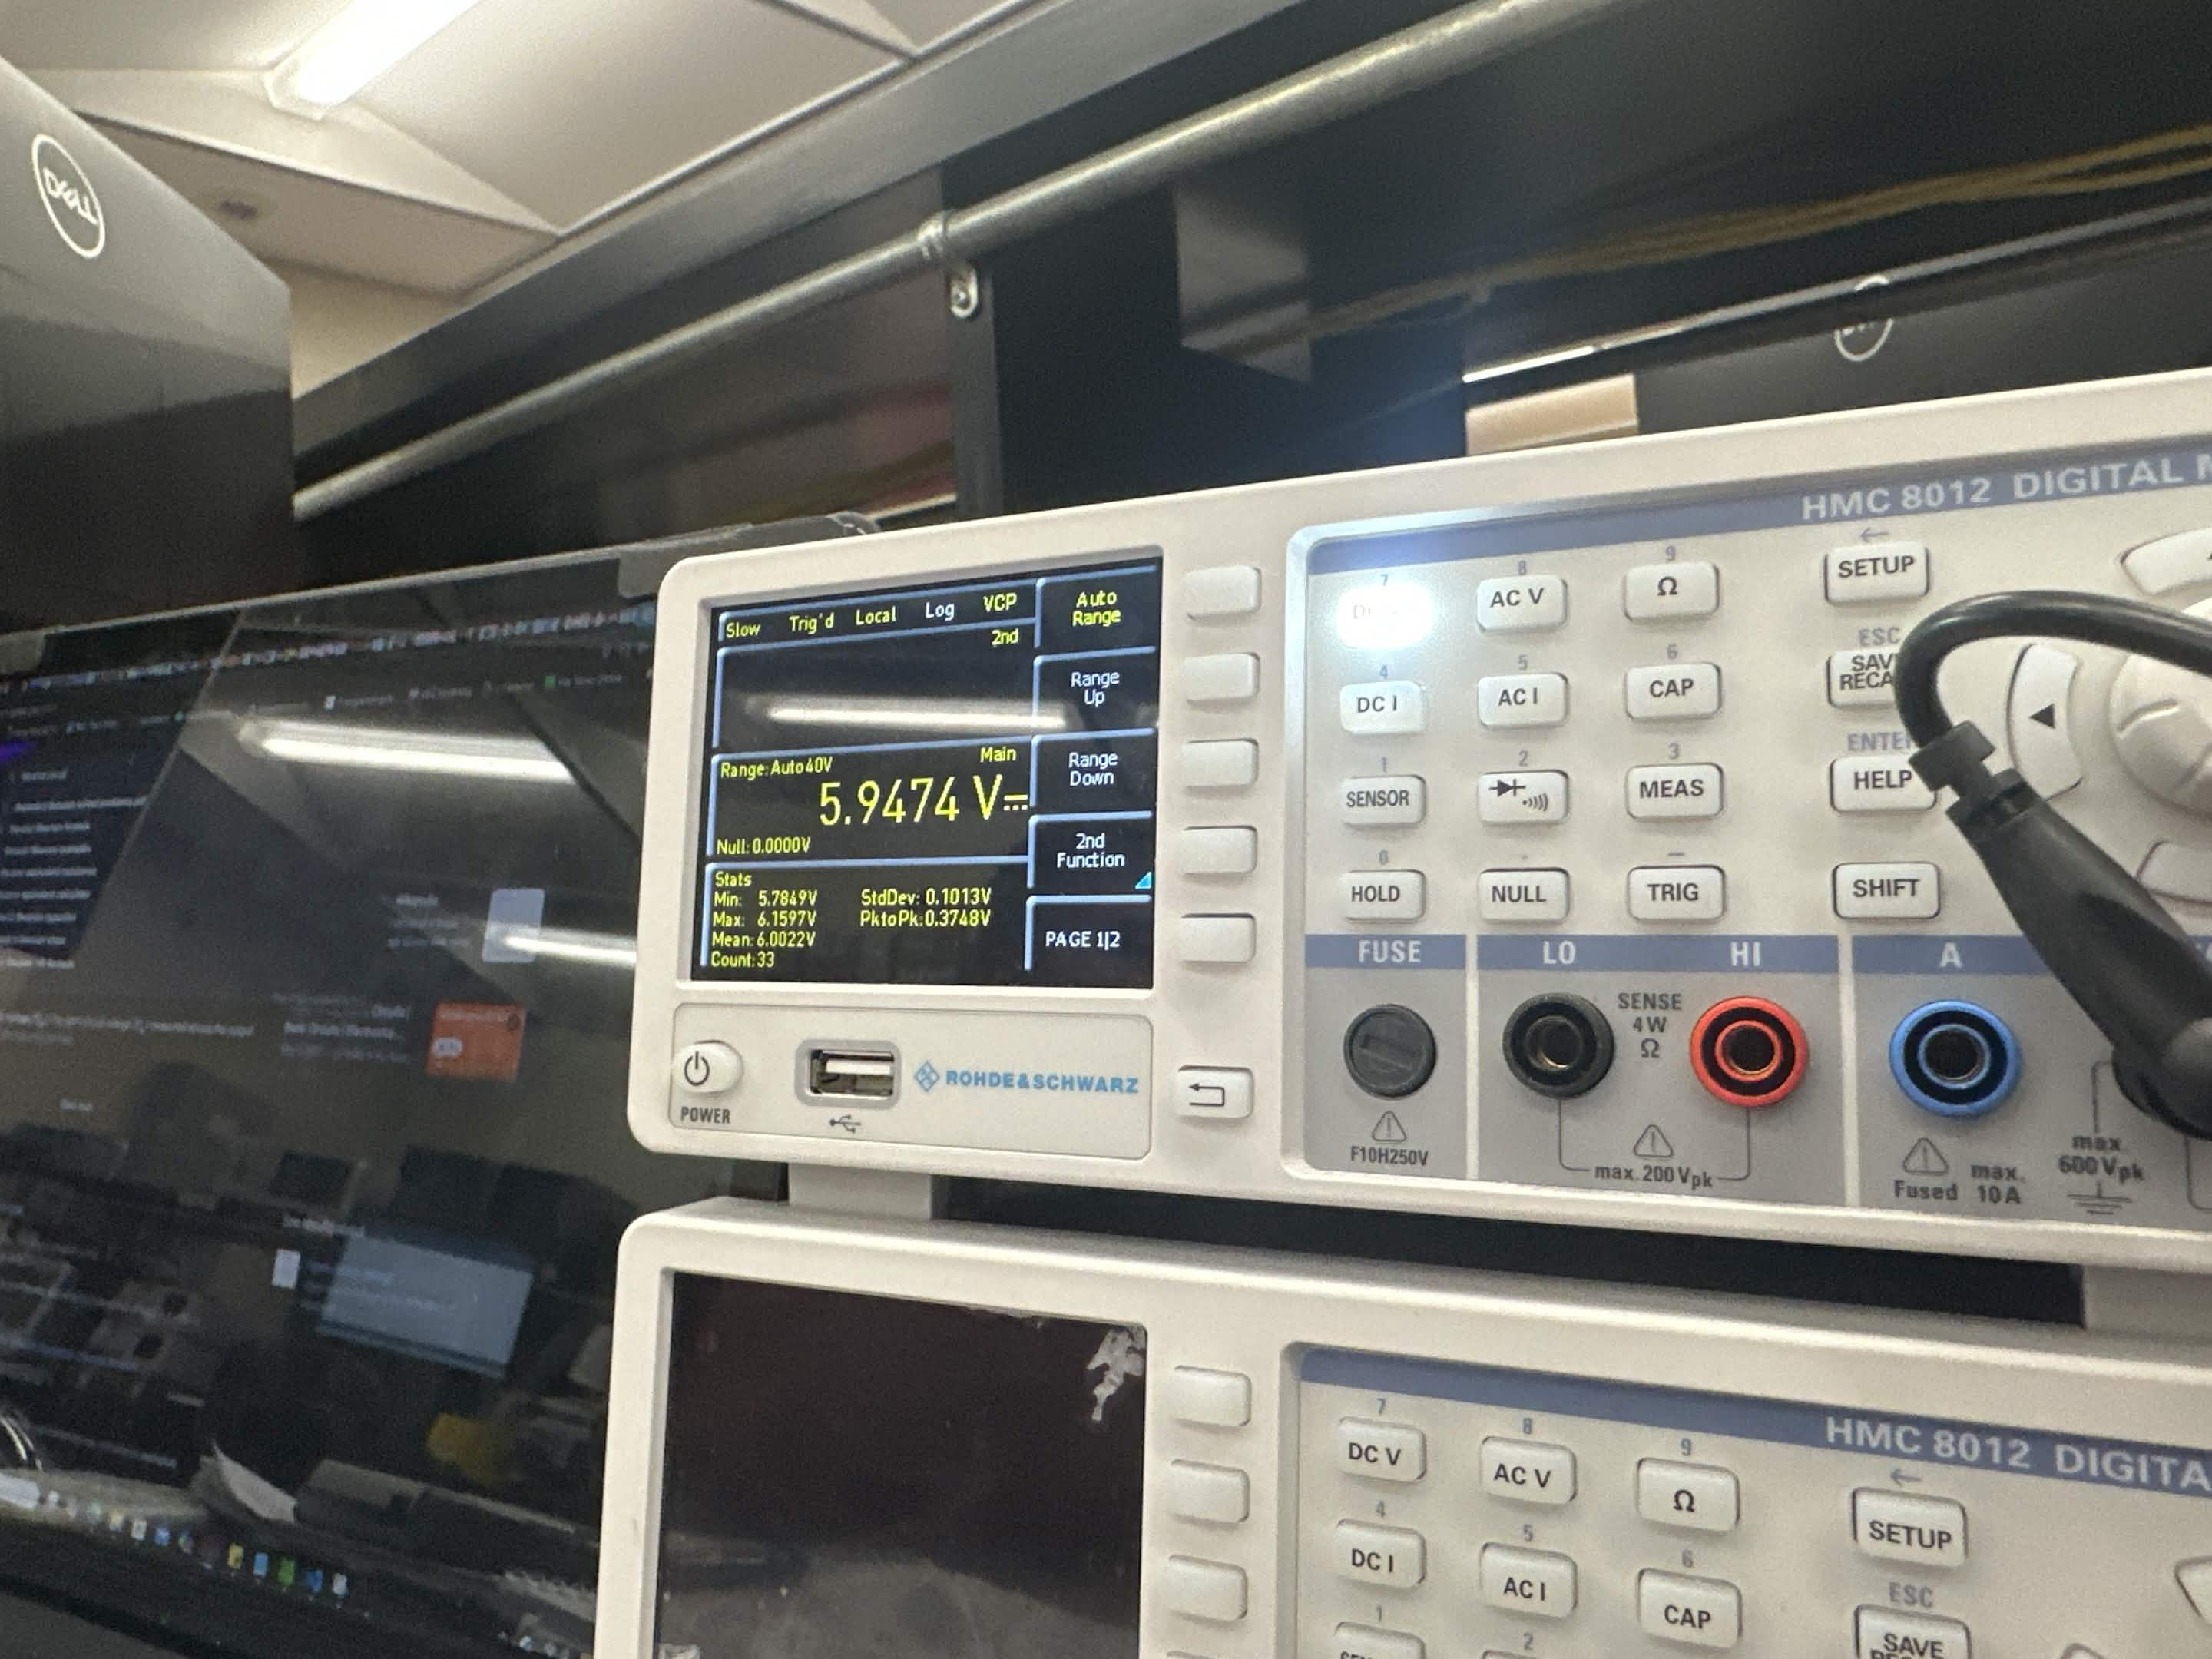
\includegraphics[width=\textwidth]{vceq_figure1b.jpg}
        \caption{Measured $V_{CEQ}$}
        \label{fig:vceq_no_re}
    \end{subfigure}
    \caption{DC operating point measurements for the bias circuit without $R_E$.}
    \label{fig:dc_bias_no_re}
\end{figure}

\pagebreak
\subsection{Transistor Biasing With Emitter Resistor (Fig. 1.b modified)}
To test bias stability, $R_E$ was introduced into the circuit. The addition of the emitter degeneration resistor provides negative feedback to stabilize the operating point against variations in $\beta$. The measured current dropped to $0.1054 \text{ mA}$, and the measured voltage shifted to $11.0485 \text{ V}$, reflecting the shift in the DC operating point caused by the unadjusted $V_{BB}$ source.

\begin{figure}[H]
    \centering
    \begin{subfigure}[b]{0.48\textwidth}
        \centering
        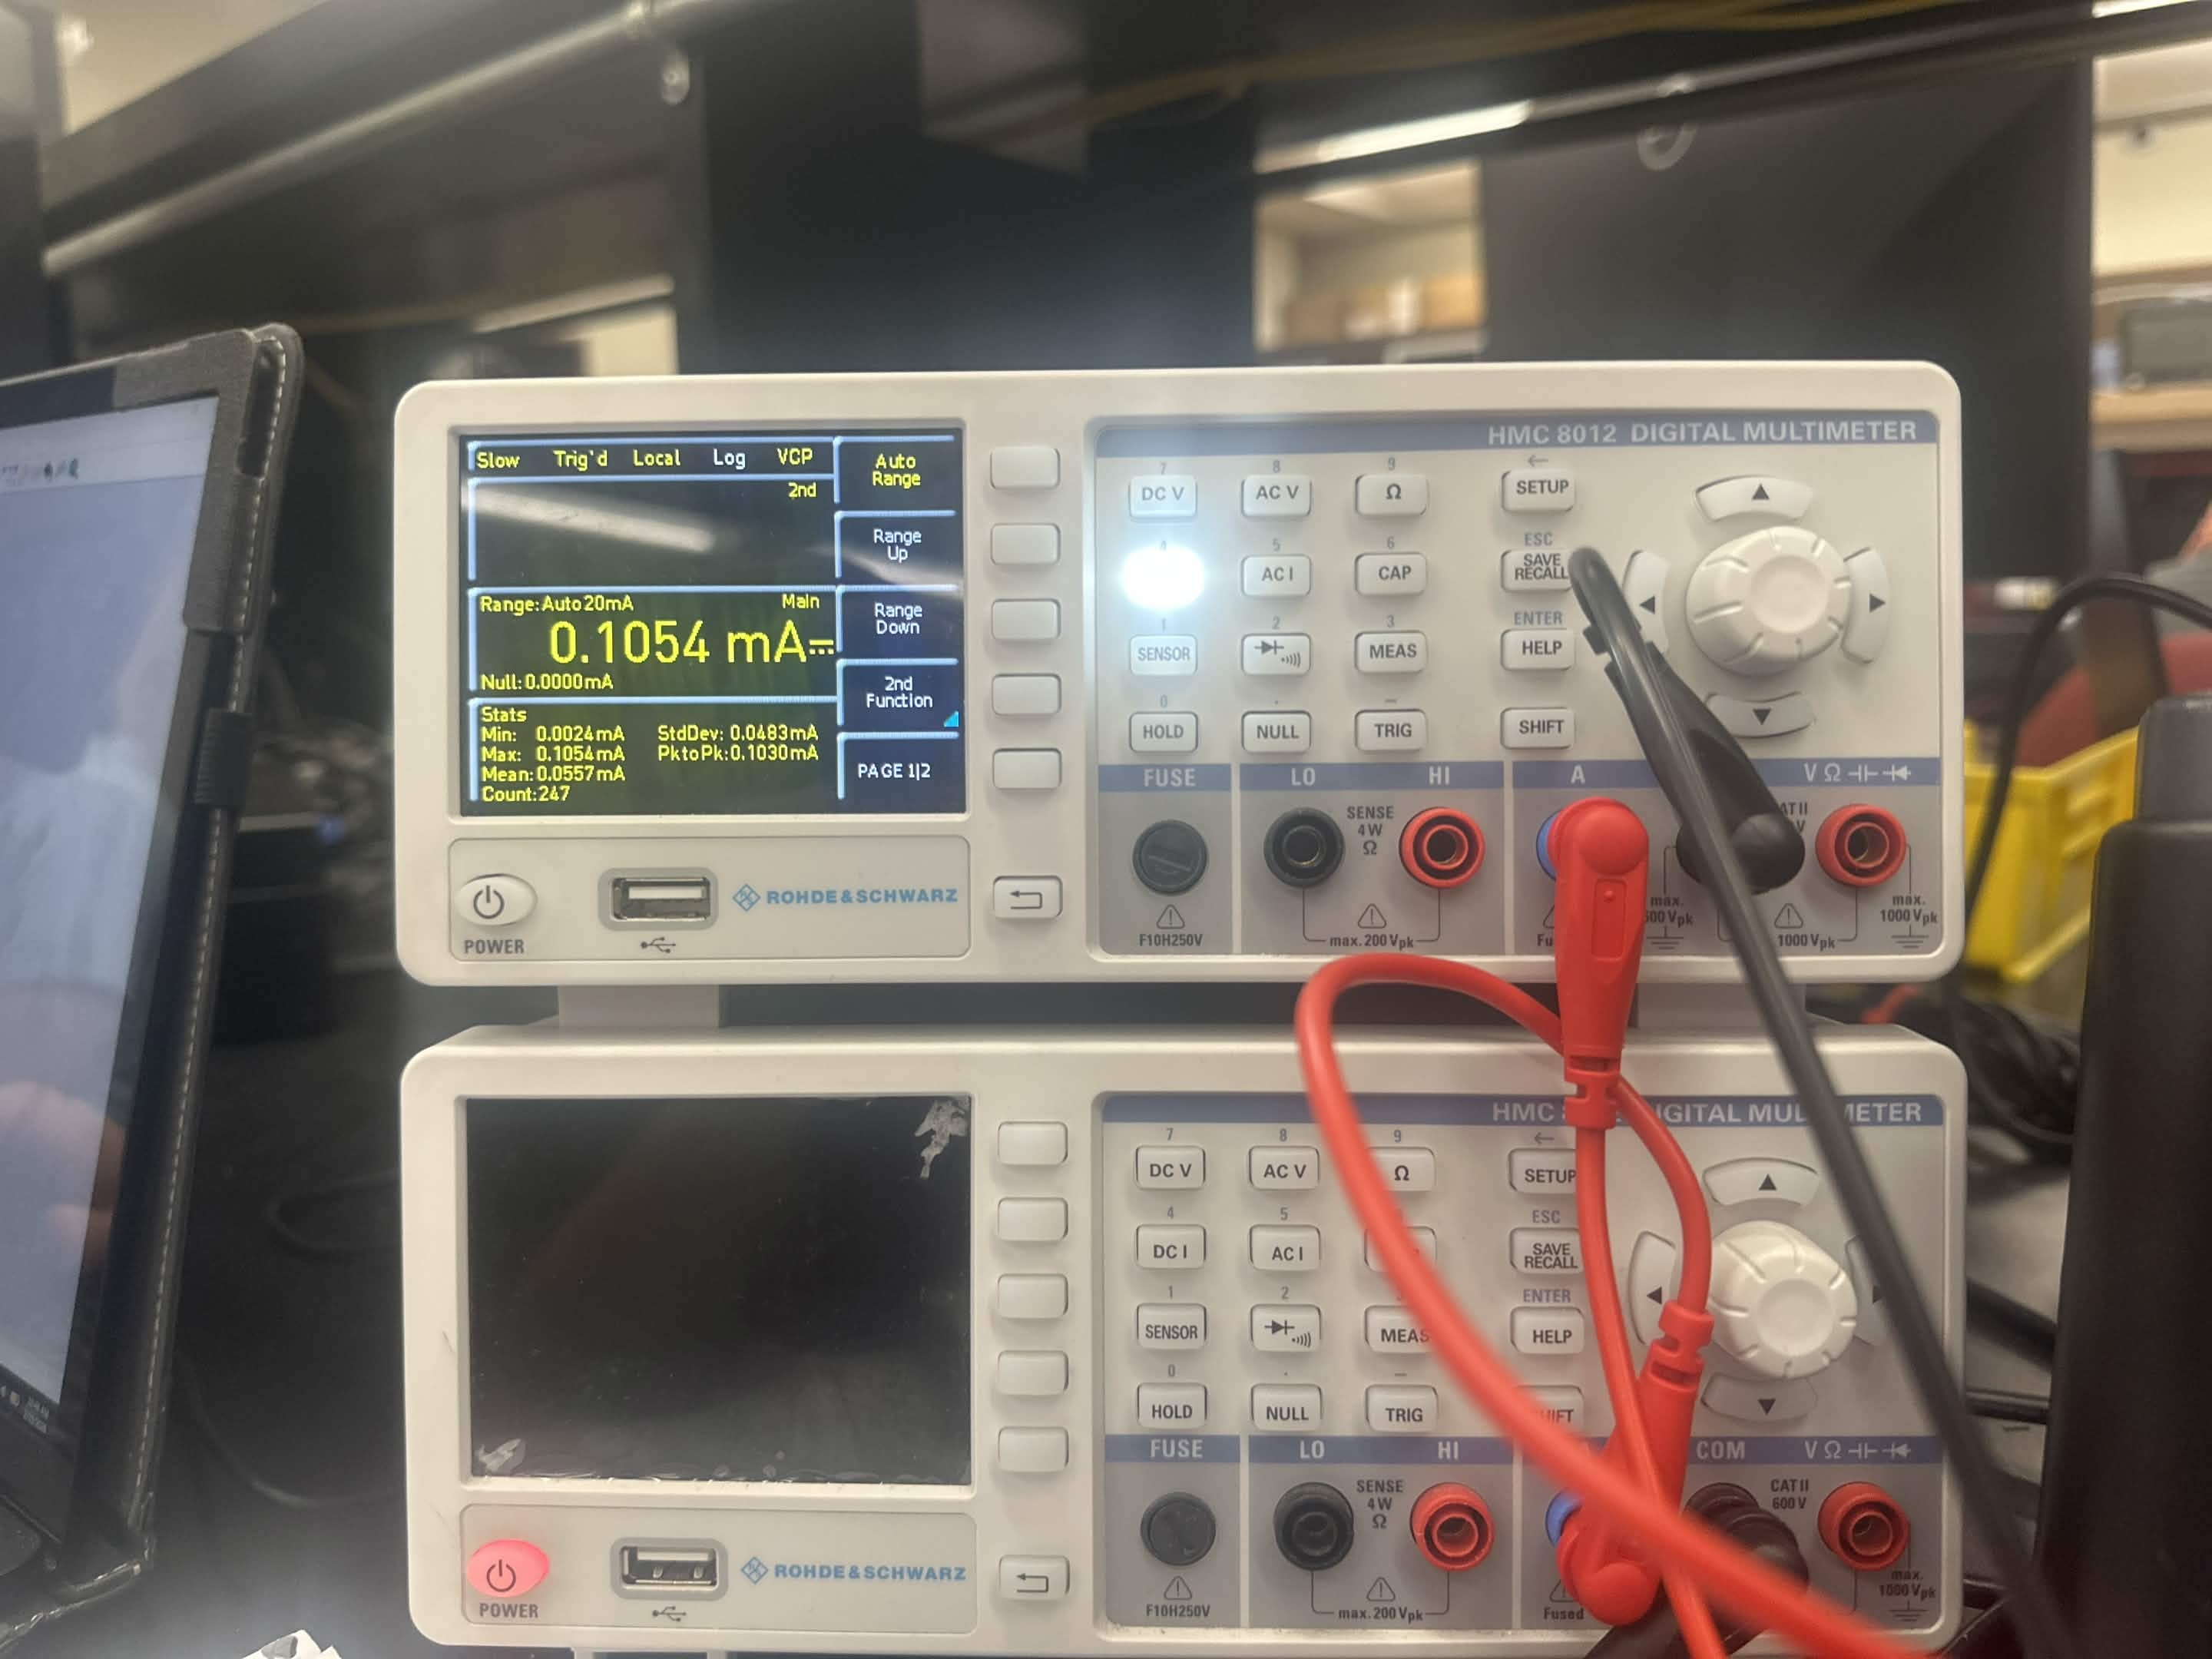
\includegraphics[width=\textwidth]{icq_with_re_figure1b.jpg}
        \caption{Measured $I_{CQ}$ with $R_E$}
        \label{fig:icq_re}
    \end{subfigure}
    \hfill
    \begin{subfigure}[b]{0.48\textwidth}
        \centering
        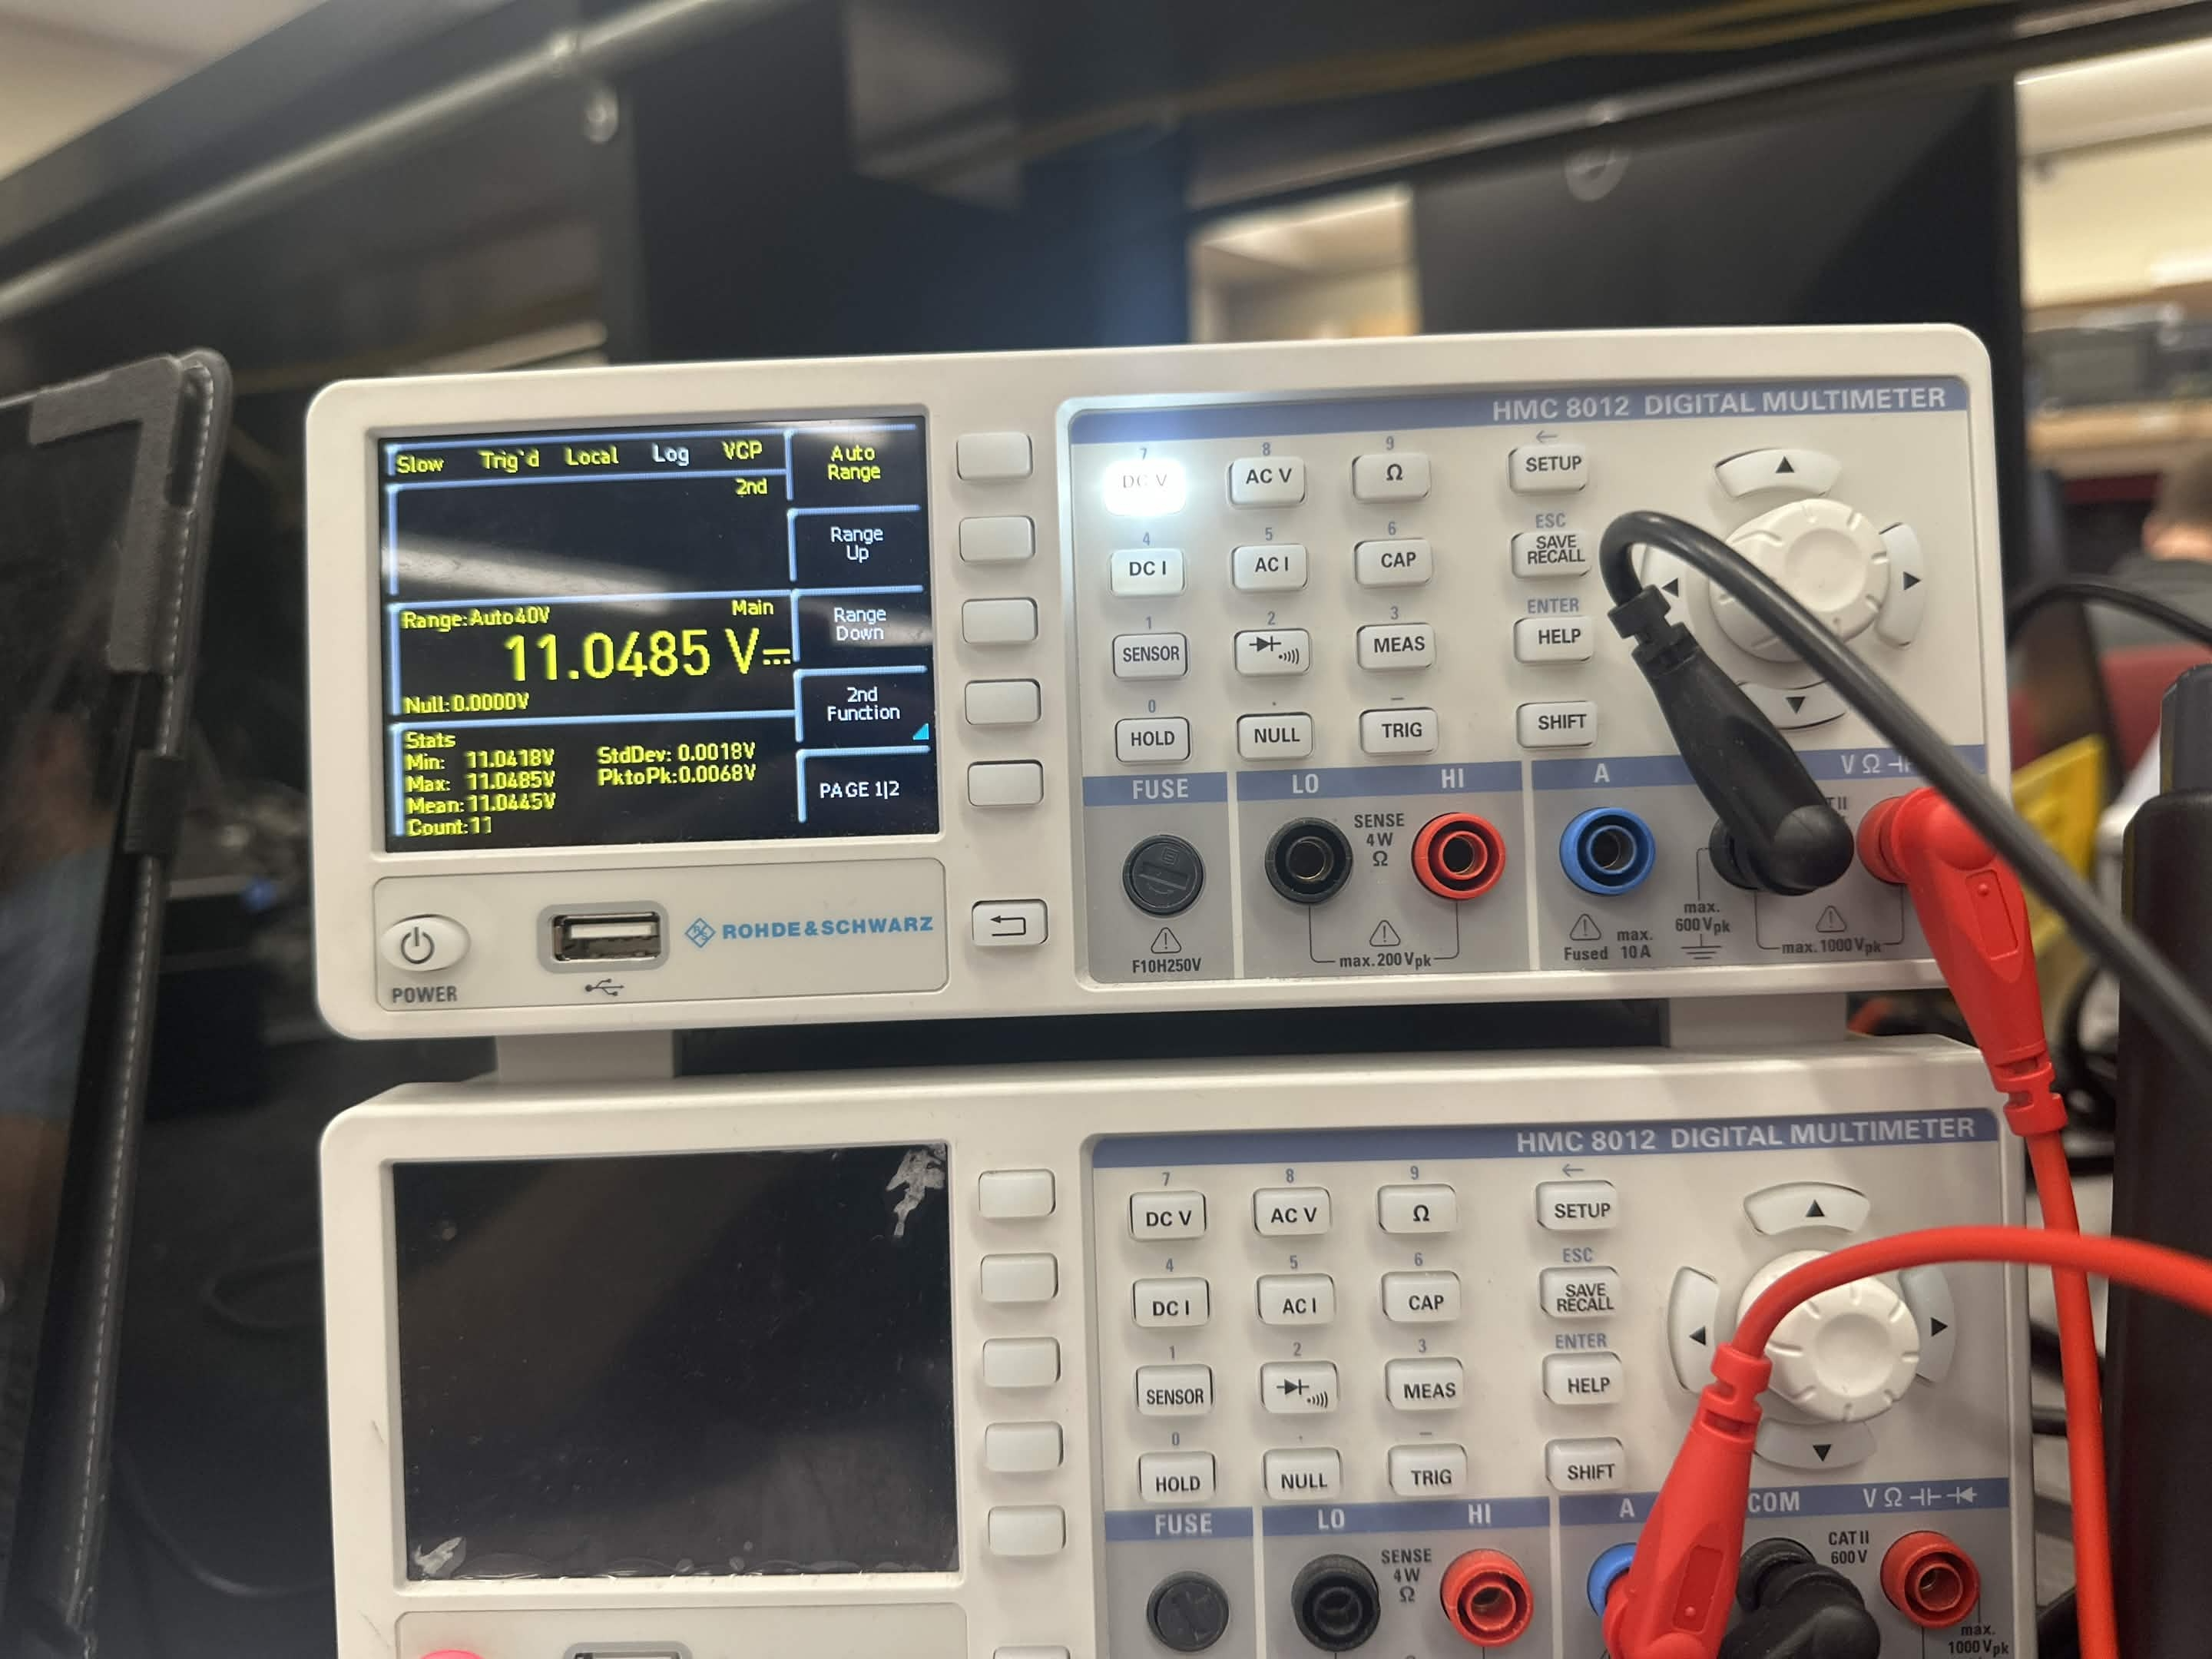
\includegraphics[width=\textwidth]{veq_with_re_figure1b.jpg}
        \caption{Measured Voltage with $R_E$}
        \label{fig:veq_re}
    \end{subfigure}
    \caption{DC measurements after introducing the emitter resistor $R_E$.}
    \label{fig:dc_bias_re}
\end{figure}

\subsection{AC Amplifier Performance (Fig. 3)}
With the voltage-divider bias circuit fully constructed and a $3 \text{ kHz}$ AC signal applied, oscilloscope traces were captured for the input voltage ($v_i$), collector voltage ($v_c$), and emitter voltage ($v_e$). The waveforms show successful small-signal amplification without clipping.

\begin{figure}[H]
    \centering
    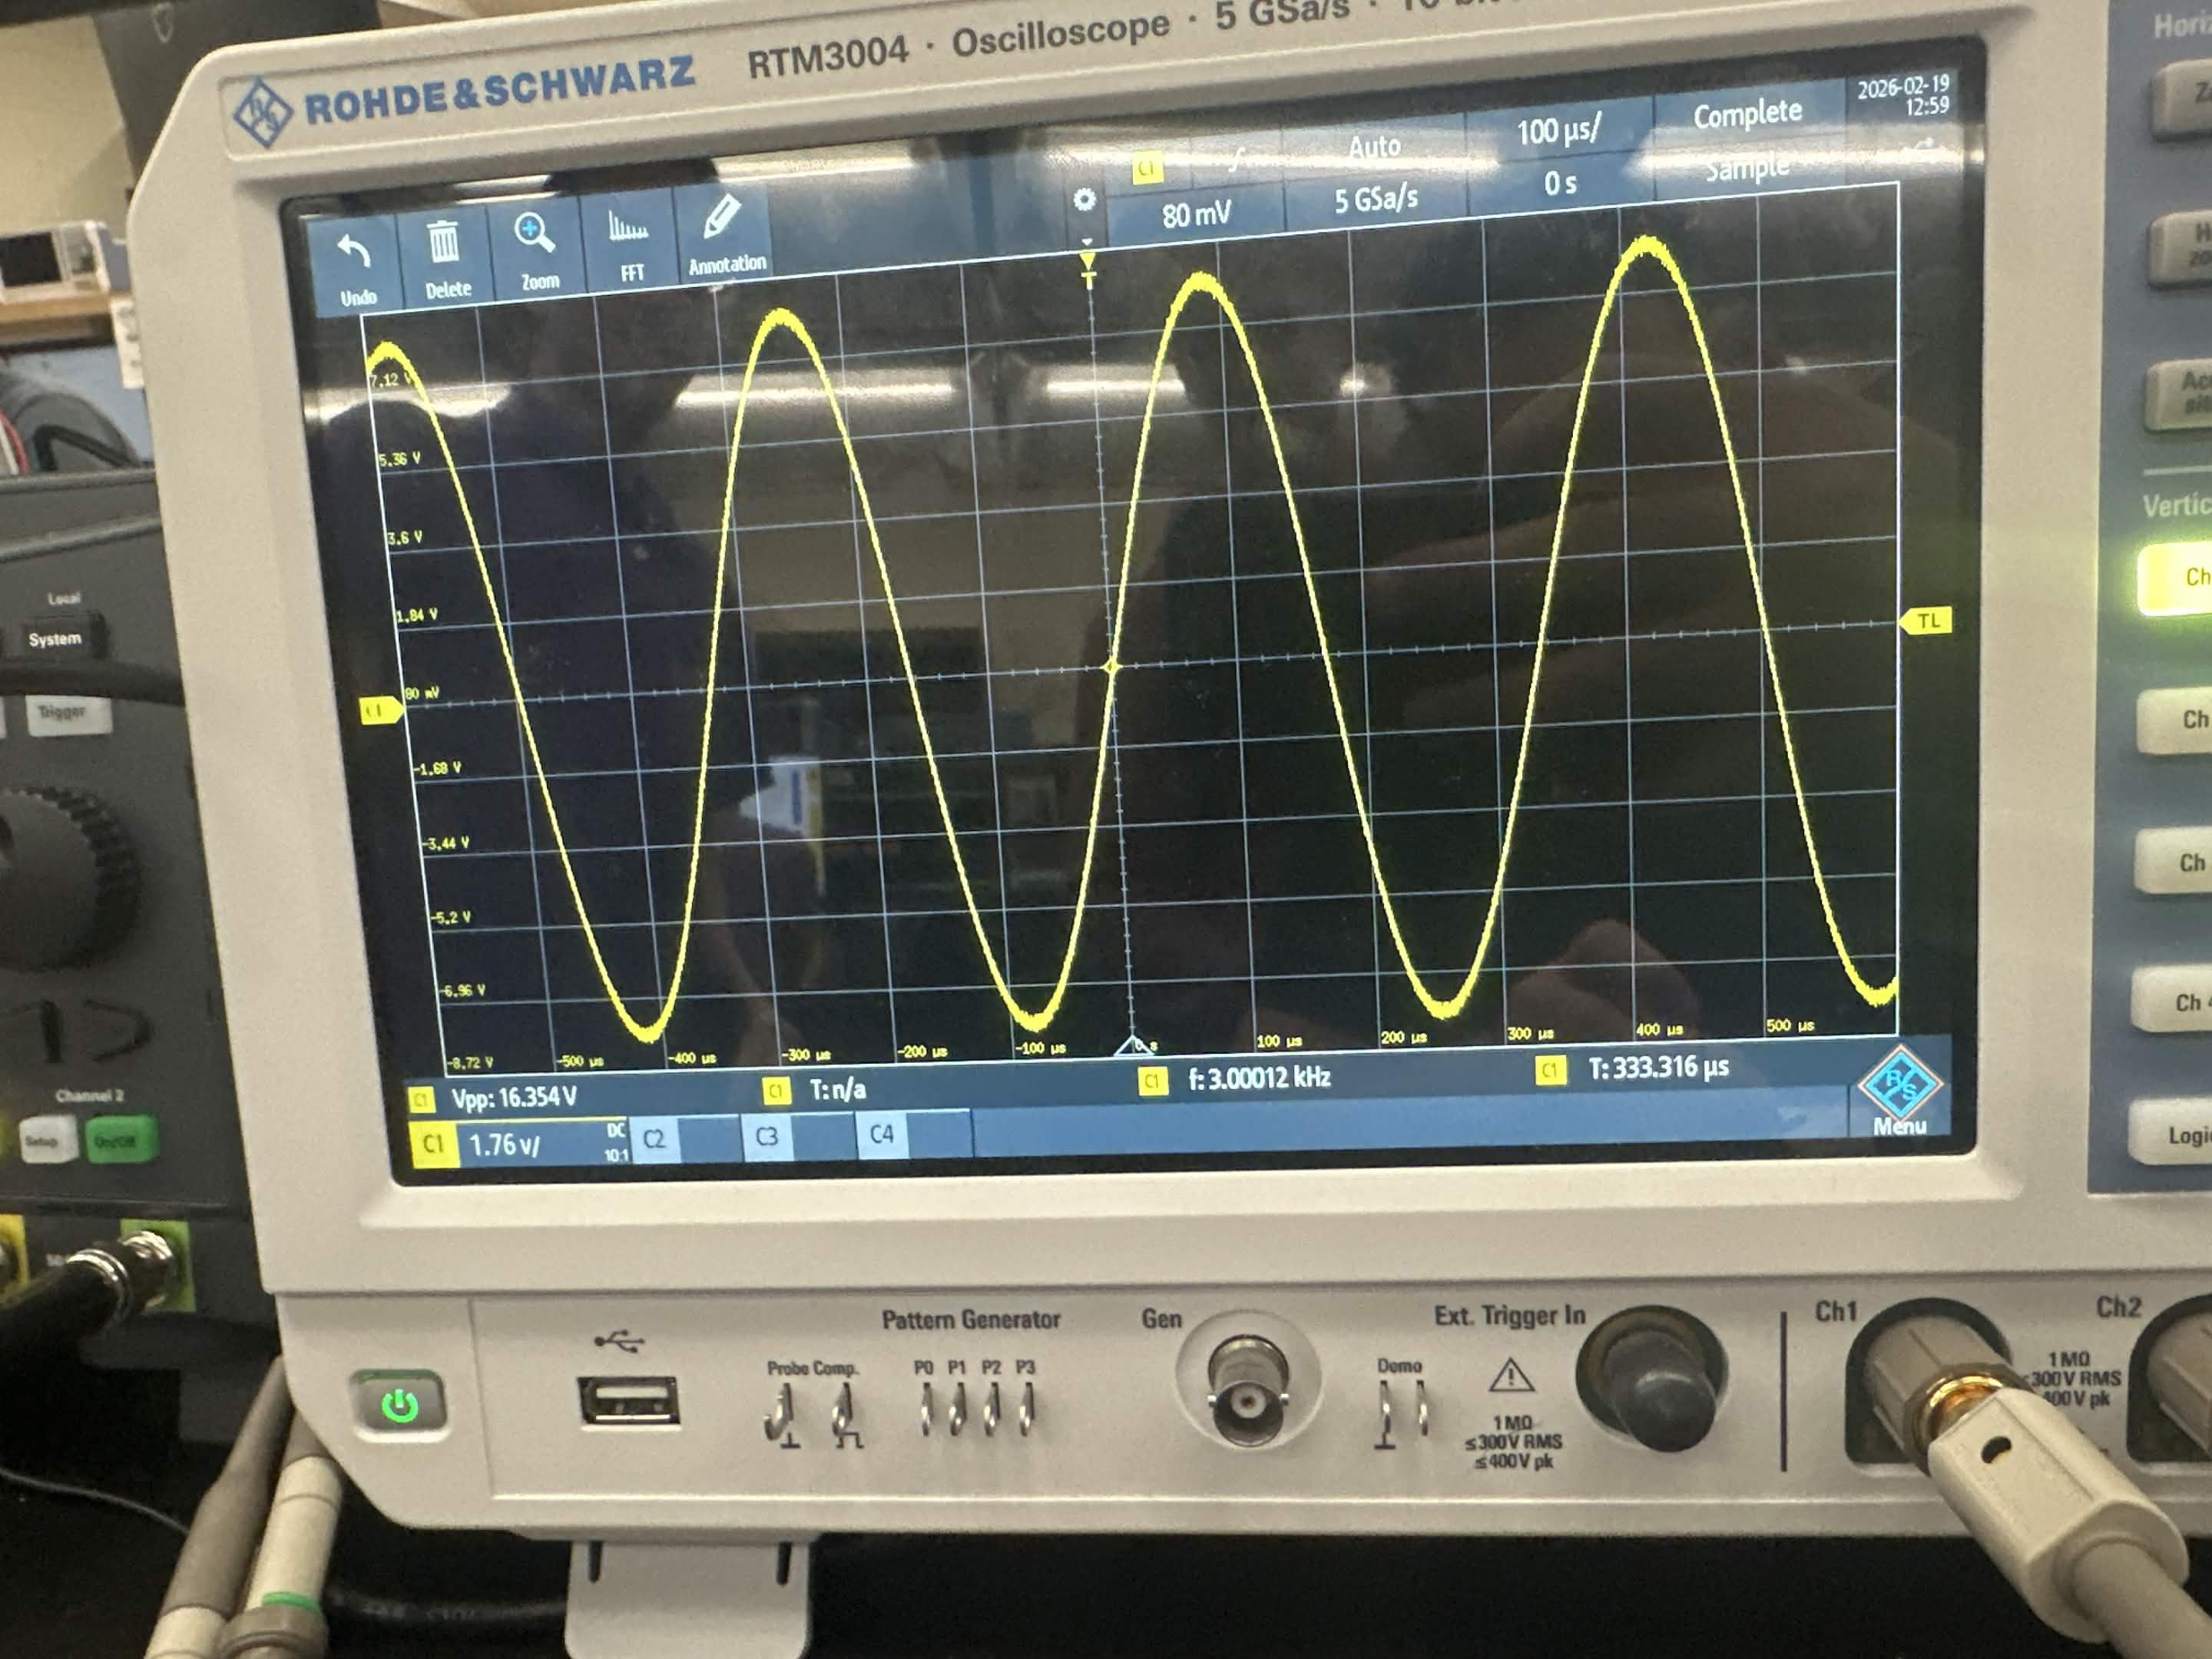
\includegraphics[width=0.55\textwidth]{vi_figure3.jpg}
    \caption{Oscilloscope capture of the input voltage waveform ($v_i$).}
    \label{fig:vi_ac}
\end{figure}

\begin{figure}[H]
    \centering
    \begin{subfigure}[b]{0.48\textwidth}
        \centering
        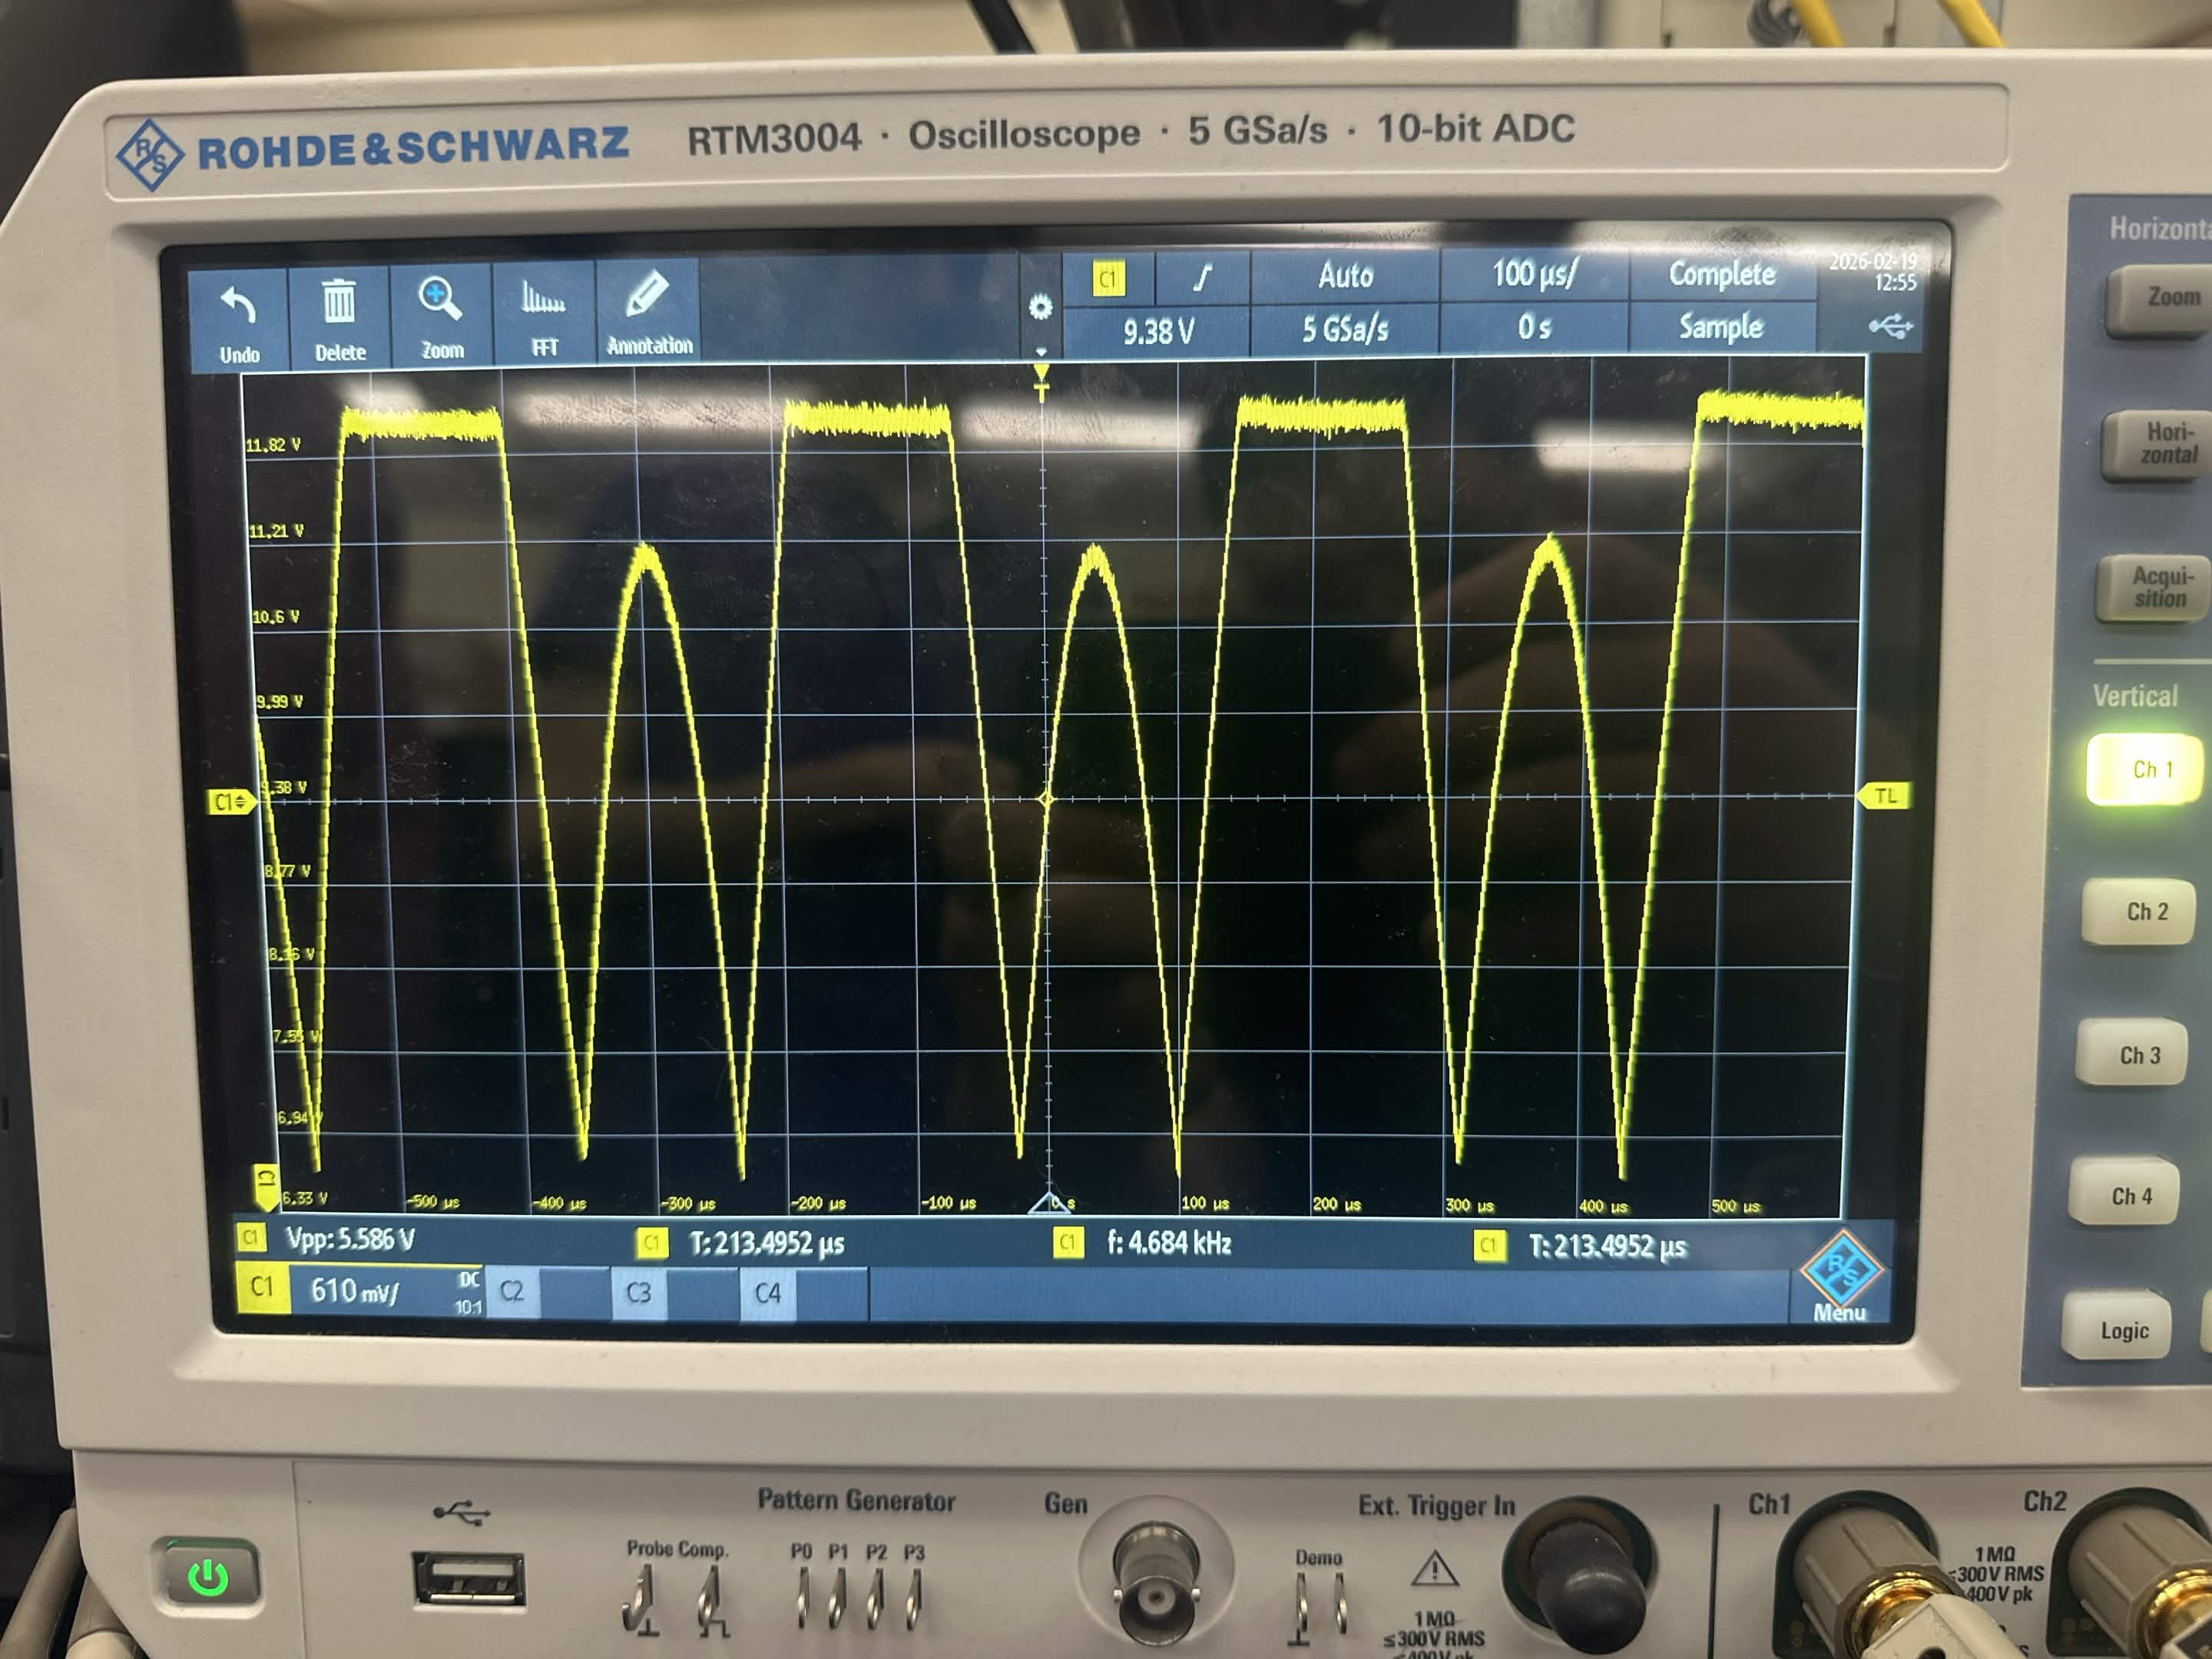
\includegraphics[width=\textwidth]{vc_figure3.jpg}
        \caption{Collector voltage waveform ($v_c$)}
        \label{fig:vc_ac}
    \end{subfigure}
    \hfill
    \begin{subfigure}[b]{0.38\textwidth}
        \centering
        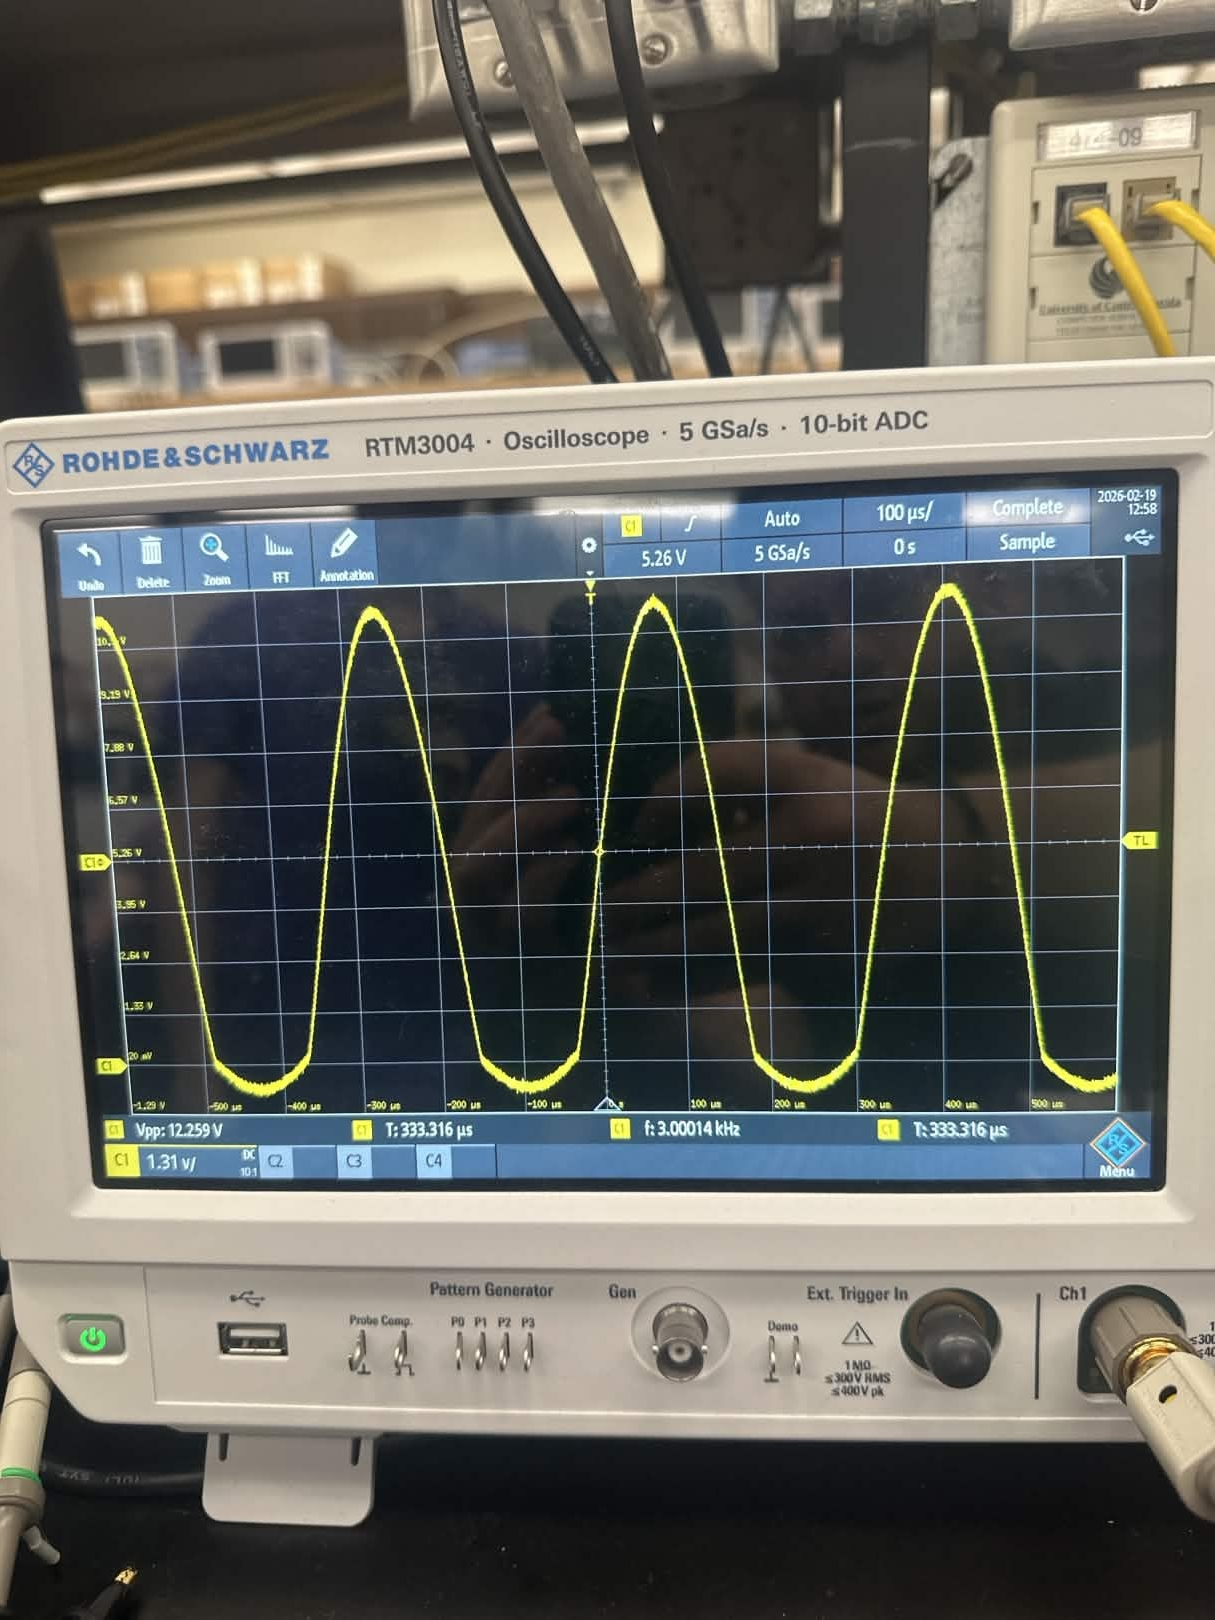
\includegraphics[width=\textwidth]{ve_figure3.jpg}
        \caption{Emitter voltage waveform ($v_e$)}
        \label{fig:ve_ac}
    \end{subfigure}
    \caption{Output voltage waveforms for the AC amplifier circuit.}
    \label{fig:outputs_ac}
\end{figure}

%----------------------------------------------------------------------------------------
%	4. PRE-LABORATORY CALCULATIONS
%----------------------------------------------------------------------------------------
\section{Pre-Laboratory Calculations}
The hand-calculated pre-laboratory derivations are attached below. All results found above and below were thankfully equivalent with the circuit simulations that I did to verify the hand calculations and waveforms.
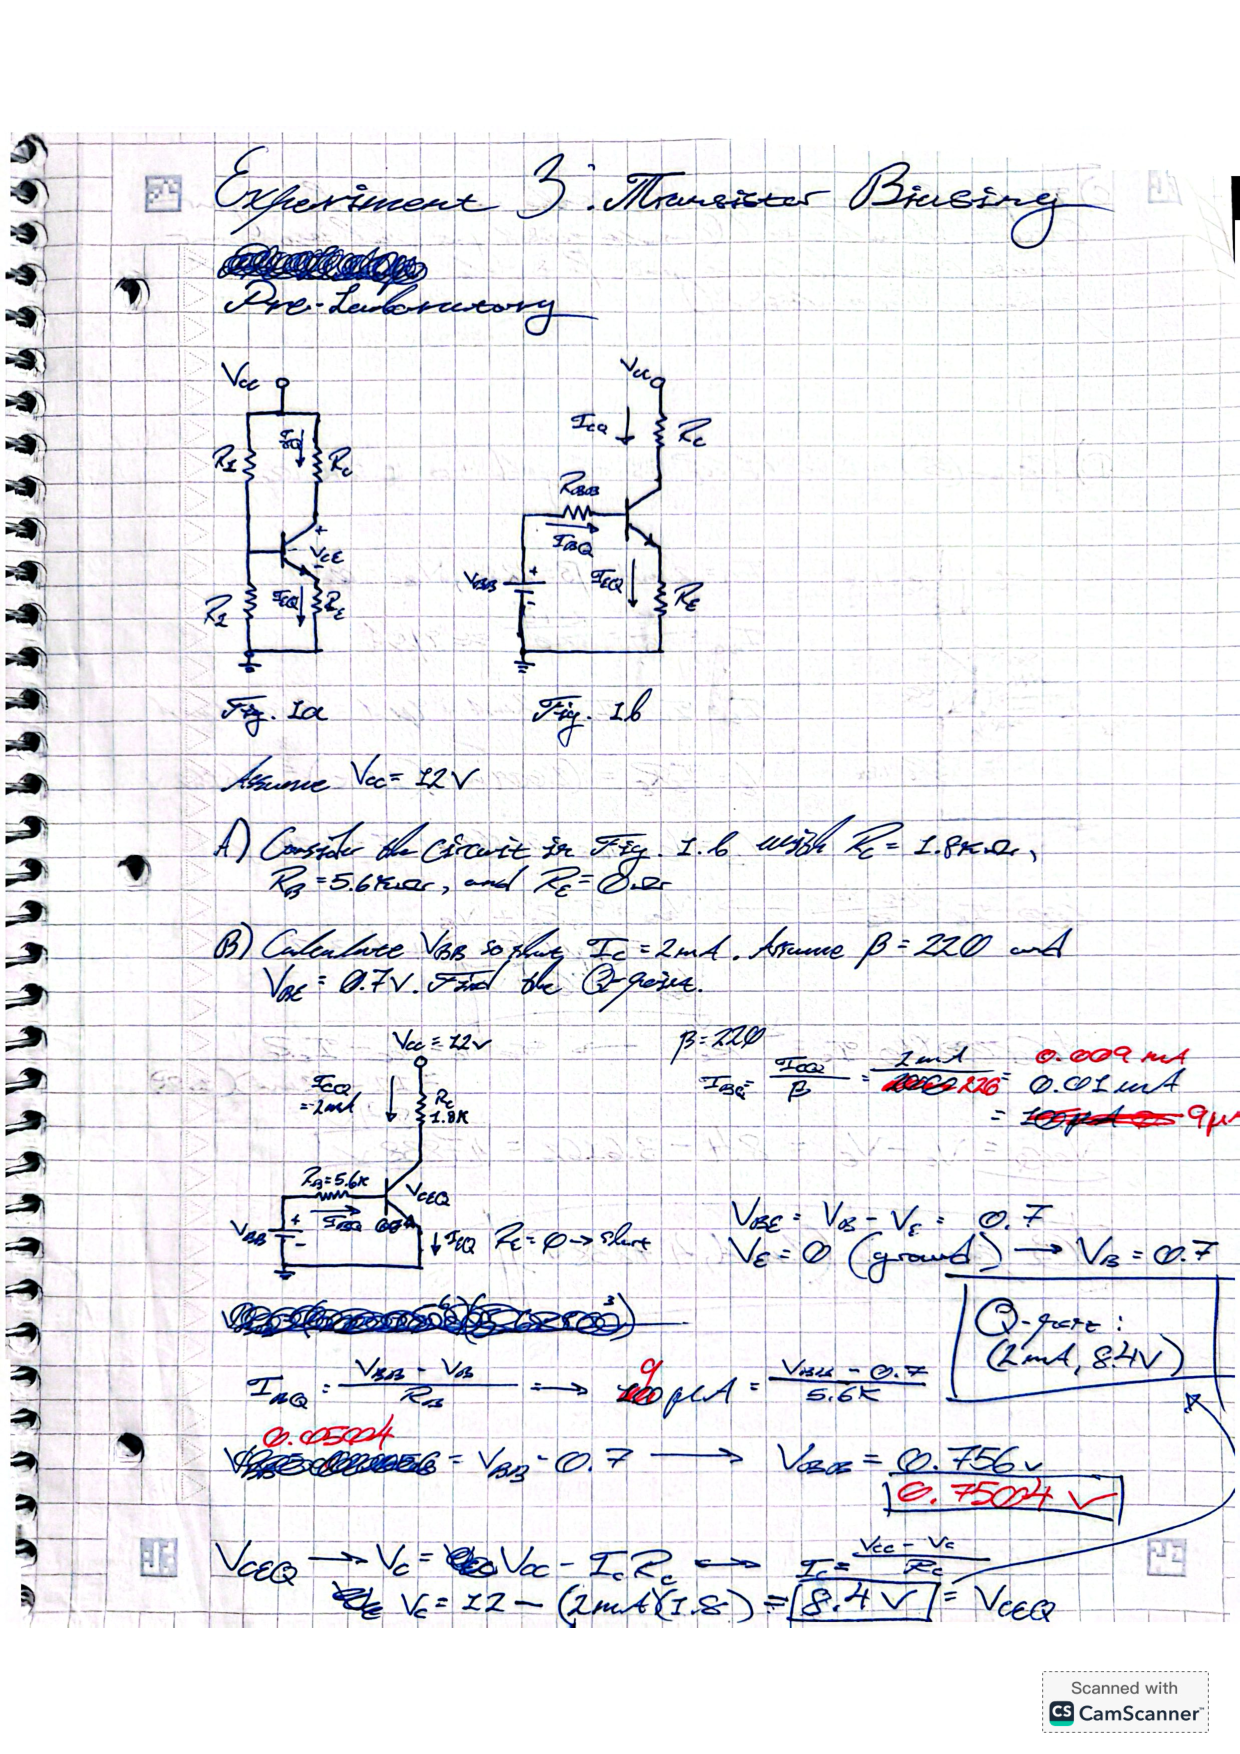
\includepdf[pages=-]{CamScanner 4-3-26 18.44.pdf}

%----------------------------------------------------------------------------------------
%	5. CONCLUSION
%----------------------------------------------------------------------------------------
\section{Conclusion}
This experiment successfully demonstrated the principles of transistor biasing and the differences between fixed-bias and emitter-stabilized bias circuits. The inclusion of $R_E$ noticeably altered the DC Q-point, highlighting the impact of emitter degeneration on circuit stability. Furthermore, the voltage-divider configuration effectively amplified the $3 \text{ kHz}$ sinusoidal signal, validating the theoretical models constructed during the pre-lab.

\end{document}
